\chapter{Analisa}

Pada bab ini, akan dilakukan analisa terhadap data yang akan diproses menggunakan \textsl{data mining} dan perangkat lunak yang akan dibangun untuk melakukan proses data tersebut.

\section{Analisis Data}
\label{analisisData}
Pada bab ini, akan dilakukan analisa \textsl{preprocessing data} yang meliputi \textsl{data cleaning}, \textsl{data integration}, \textsl{data selection} dan \textsl{data transformation}. Setelah membaca dan menganalisis data \textsl{log} histori KIRI, maka penelitian ini akan lebih fokus untuk meneliti mengenai lokasi keberangkatan dan tujuan dari user yang menggunakan aplikasi KIRI.

\subsection{Data Cleaning}
Pada tahap ini, data yang akan menjadi input akan diperiksa apakah mengandung \textsl{missing value} atau \textsl{noisy}. Setelah dilakukan pemeriksaan, tidak ditemukan \textsl{missing value} ataupun \textsl{noisy}, sehingga tahap ini dapat dilewat.

\subsection{Data Integration}
Pada tahap ini, data-data dari beberapa database akan digabung dan diintegrasikan menjadi satu database. Karena data yang digunakan hanya berasal dari satu tabel, maka tahap ini dapat dilewat.

\subsection{\textsl{Data Selection}}
Pada tahap ini, akan dilakukan pemilihan data yang akan digunakan. Pada penelitian ini, akan dilakukan proses \textsl{data mining} mengenai lokasi keberangkatan dan tujuan dari seorang user yang menggunakan aplikasi KIRI. Oleh karena itu, pada atribut \textsl{action}, nilai yang akan dipilih hanya \textsl{FINDROUTE}. Hal ini dikarenakan, hanya \textsl{action FINDROUTE} yang menjelaskan posisi keberangkatan dan tujuan dari user. Selain itu, data tersebut terlihat menarik karena dimungkinkan dapat menghasilkan suatu pola yang membantu melakukan klasifikasi mengenai perpindahan penduduk khususnya untuk daerah Bandung. Karena seluruh \textsl{action} bernilai satu jenis yaitu \textsl{FINDROUTE}, maka atribut tersebut dapat dihilangkan. Selain itu, atribut logId dan APIKey tidak akan dimasukan ke dalam proses karena tidak memiliki hubungan dengan lokasi keberangkatan dan tujuan dari seorang user.

Dari analisis diatas, maka atribut yang dipilih untuk diproses ke dalam \textsl{data mining} adalah
\begin{itemize}
	\item \textsl{Timestamp} (UTC)
	\item \textsl{AdditionalData}
\end{itemize}

Berikut contoh data dari atribut tersebut dapat dilihat pada tabel \ref{table:contohDataLog}
\begin{table}[h]
\caption{Contoh data \textsl{log} KIRI setelah \textsl{data selection}}
\label{table:contohDataLog}
\begin{tabular}{|l|l|}
\hline
\textbf{Timestamp (UTC)} & \textbf{AdditionalData}                     \\ \hline
2/1/2014 0:11            & -6.8972513,107.6385574/-6.91358,107.62718/1 \\ \hline
2/1/2014 0:13            & -6.8972513,107.6385574/-6.91358,107.62718/1 \\ \hline
2/1/2014 0:16            & -6.90598,107.59714/-6.90855,107.61082/1     \\ \hline
2/1/2014 0:18            & -6.9015366,107.5414474/-6.88574,107.53816/1 \\ \hline
2/1/2014 0:25            & -6.90608,107.61530/-6.89140,107.61060/2     \\ \hline
2/1/2014 0:27            & -6.89459,107.58818/-6.89876,107.60886/2     \\ \hline
2/1/2014 0:28            & -6.89459,107.58818/-6.86031,107.61287/2     \\ \hline
\end{tabular}
\end{table}

Pada atribut \textsl{additionalData}, jika nilai atribut \textsl{action} adalah \textsl{FINDROUTE}, maka nilai \textsl{additionalData} memiliki tiga bagian yang dibatasi dengan '/'. Ketiga bagian tersebut adalah

\begin{enumerate}
	\item Nilai latitude dan longitude dari lokasi keberangkatan yang dipilih oleh user
	\item Nilai latitude dan longitude dari lokasi tujuan yang dipilih oleh user
	\item Nilai yang menunjukkan banyak jalur yang dihasilkan oleh sistem KIRI
\end{enumerate}

Nilai dari banyak jalur akan dibuang ketika memasuki tahap \textsl{data transformation}, karena nilai tersebut hanya menunjukkan banyak jalur tetapi user pasti hanya memilih salah satu dari jalur tersebut, sehingga nilai jalur ini dapat diasumsikan memiliki nilai 1 semua. karena kolom jalur bernilai satu semua, maka kolom tersebut dapat dibuang.

\subsection{\textsl{Data Transformation}}
Pada tahap ini, akan dilakukan perubahan data. Pada atribut yang dipilih, nilai dari atribut \textsl{timestamp} dan \textsl{additionaldata} perlu dilakukan transformasi agar program dapat membaca dan memproses data lebih cepat. 

Pada atribut \textsl{timestamp}, nilai waktu dari atribut tersebut akan diubah menjadi waktu GMT+8. Kemudian, data akan diubah menjadi empat atribut, yaitu:
\begin{itemize}
	\item Bulan, atribut ini akan menunjukkan bulan ketika user KIRI memanggil \textsl{action FINDROUTE}, dengan nilai antara 01 sampai 12. Nilai tersebut dapat diperoleh dengan cara mengambil nilai string dari timpestamp yang berada di antara garis miring pertama dan kedua.
	\item Tahun, atribut ini akan menunjukkan tahun ketika user KIRI memanggil \textsl{action FINDROUTE}, dengan format empat angka (contoh: 2014). Nilai tersebut dapat diperoleh dengan cara mengambil nilai string dari timpestamp yang berada di antara garis miring kedua dan spasi.
	\item Hari, atribut ini akan menunjukkan hari ketika user KIRI memanggil \textsl{action FINDROUTE}, dengan range nilai antara senin sampai minggu. Nilai tersebut dapat diperoleh dengan cara melakukan memanggil \textsl{method} pencarian hari berdasarkan tanggal dari timestamp pada java.
	\item Jam, atribut ini akan menunjukkan jam ketika user KIRI memanggil \textsl{action FINDROUTE}, dengan range nilai antara 00 sampai 23. Nilai tersebut dapat diperoleh dengan cara mengambil nilai string dari timpestamp yang berada di antara spasi dan titik dua.
\end{itemize}

Data \textsl{timestamp} diubah menjadi enam bagian, agar dapat dilakukan pengelompokan yang dilihat dari tanggal, bulan, tahun, hari, jam dan menit.

Pada atribut \textsl{additionalData}, data akan diubah menjadi empat atribut, yaitu:
\begin{itemize}
	\item Latitude keberangkatan, atribut ini berisi nilai latitude dari lokasi keberangkatan yang dipilih oleh user. Nilai tersebut dapat diperoleh dengan cara mengambil nilai string sebelum koma yang pertama.
	\item Longitude keberangkatan, atribut ini berisi nilai longitude dari lokasi keberangkatan yang dipilih oleh user. Nilai tersebut dapat diperoleh dengan cara mengambil nilai string yang berada di antara koma pertama dan garis miring pertama.
	\item Latitude tujuan, atribut ini berisi nilai latitude dari lokasi tujuan yang dipilih oleh user. Nilai tersebut dapat diperoleh dengan cara mengambil nilai string di antara garis miring yang pertama dan koma kedua.
	\item Longitude tujuan, atribut ini berisi nilai longitude dari lokasi tujuan yang dipilih oleh user. Nilai tersebut dapat diperoleh dengan cara mengambil nilai string yang berada di antara koma kedua dan garis miring kedua.
\end{itemize}

Data \textsl{additionalData} diubah menjadi empat bagian, agar program dapat membaca data tersebut lebih mudah.

Dari analisis diatas, banyak atribut dari tabel \textsl{statistics} akan menjadi delapan, yaitu:
\begin{itemize}
	\item Bulan
	\item Tahun
	\item Hari
	\item Jam
	\item Latitude Keberangkatan
	\item Longitude Keberangkatan
	\item Latitude Tujuan
	\item Longitude Tujuan
\end{itemize}

Contoh hasil data transformasi jika input merupakan data dari tabel \ref{table:contohDataLog} dapat dilihat pada tabel \ref{table:contohHasilDataTransformasi}	.

\begin{center}
\begin{table}
\rotatebox{90}{%
%\begin{tabular}{|@{}>{\raggedright}p{.2\textheight}>{\raggedright}p{.2\textheight}>{\raggedright}p{.2\textheight}>{\raggedright\arraybackslash}p{.2\textheight}@{}|
\begin{tabular}{|l|l|l|l|p{2.5cm}|p{2.5cm}|p{2.5cm}|p{2.5cm}|}
\hline
\textbf{Bulan}	& \textbf{Tahun} 	& \textbf{Hari} & \textbf{Jam} & \textbf{Latitude Keberangkatan} & \textbf{Longitude Keberangkatan} & \textbf{Latitude Tujuan} & \textbf{Longitude Tujuan}      \\ \hline
02								& 2014						& Sabtu         & 00						 & -6.8972513										 & 107.6185574 							  & -6.91358                & 107.62718 \\ \hline
02								& 2014						& Sabtu         & 00						 & -6.8972513										 & 107.6385574                & -6.91358							  & 107.62718 \\ \hline
02								& 2014						& Sabtu         & 00 						 & -6.90598											 & 107.59714     		  				& -6.90855						&107.61082 \\ \hline
02								& 2014						& Sabtu         & 00  					 & -6.9015366										 & 107.5414474 								& -6.88574					    & 107.53816 \\ \hline
02								& 2014						& Sabtu         & 00 						 & -6.90608										   & 107.61530     						  & -6.89140					 &107.61060 \\ \hline
02								& 2014						& Sabtu         & 00 						 & -6.89459											 & 107.58818     							& -6.89876						&107.60886 \\ \hline
02								& 2014						& Sabtu         & 00 						 & -6.89459											 &107.58818  								   & -6.86031					 &107.61287 \\ \hline
\end{tabular}%
}
\caption{Contoh hasil data transformasi}
\label{table:contohHasilDataTransformasi}
\end{table}
\end{center}

Agar dapat diperoleh \textsl{decision tree} mengenai lokasi keberangkatan dan tujuan dari user KIRI, maka atribut kelas yang akan digunakan adalah nilai latitude dan longitude dari lokasi keberangkatan dan tujuan. Karena atribut kelas ada empat, maka akan dilakukan penyederhanaan dari keempat atribut untuk meningkatkan akurasi serta tingkat efisien proses \textsl{data mining}. 

Nilai \textsl{latitude} serta \textsl{longitude} dari data lokasi keberangkatan dan tujuan akan diubah menjadi nilai yang menunjukkan apakah daerah lokasi keberangkatan dan tujuan tersebut menunjukkan perjalanan keluar dari Bandung, menuju Bandung, atau menuju daerah yang sama. Hal ini dilakukan agar diperoleh data perbandingan pergerakan penduduk, apakah mereka lebih banyak yang keluar dari Bandung atau sebaliknya atau bahkan menuju daerah yang sama berdasarkan waktu tertentu. Untuk menentukan hal tersebut, maka akan dibutuhkan klasifikasi daerah agar mudah dilakukan penentuan apakan \textsl{user} akan berangkat ke Bandung atau tidak. \textsl{Classification} daerah yang ditentukan setelah melihat peta Bandung dapat dilihat pada gambar \ref{fig:classificationMap}.

\begin{figure}
\centering
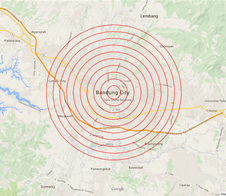
\includegraphics[scale=1]{Gambar/classificationmap.jpg}
\caption[\textsl{Classification} pada daerah Bandung]{\textsl{Classification} pada daerah Bandung}
\label{fig:classificationMap} 
\end{figure}

Penentuan \textsl{classification} tersebut berdasarkan titik pusat, yaitu -6.916667,107.6 \footnote{http://tools.wmflabs.org/geohack/geohack.php?pagename=Bandung\&params=6\_55\_S\_107\_36\_E\_region:ID-JB\_type:city} dalam latitude dan longitude. Kemudian dibagi menjadi sepuluh daerah yang memiliki perbedaan radius sebesar 1 km, sehingga diameter untuk daerah pertama adalah 2 km, diameter untuk daerah kedua adalah 4 km, dan seterusnya, untuk daerah terakhir (yaitu daerah 10) akan memiliki diameter 20 km.

Suatu lokasi atau titik latitude longitude dapat diketahui berada pada daerah yang mana dengan cara menghitung jarak titik tersebut dengan titik pusat yang sudah ditentukan (yaitu -6.916667,107.6) dengan menggunakan rumus Haversine. Jika jarak yang diperoleh lebih kecil sama dengan 1 km, maka berada di daerah pertama, sedangkan jika jarak yang diperoleh lebih kecil sama dengan 2 km dan lebih besar dari 1 km, maka berada di daerah kedua, dan seterusnya, dan untuk daerah terakhir (yaitu daerah 10) titik akan memiliki jarak lebih kecil sama dengan 10 km dan lebih besar dari 9 km dengan titik pusat. Jika suatu titik memiliki jarak terhadap titik pusat lebih dari 10 km, maka akan menjadi daerah luar Bandung.

Setelah lokasi keberangkatan dan lokasi tujuan ditentukan daerahnya, dapat ditentukan apakah user tersebut menuju pusat Bandung atau tidak. Jika daerah dari lokasi keberangkatan lebih besar daripada daerah lokasi tujuan, maka user tersebut menuju pusat Bandung. Kemudian, jika daerah dari lokasi keberangkatan lebih kecil daripada daerah lokasi tujuan, maka user tersebut tidak menuju pusat Bandung. Sedangkan, jika lokasi keberangkatan dan lokasi tujuan berada di daerah yang sama, maka user tersebut maka user tersebut bergerak di daerah yang sama.

Dengan adanya perhitungan jarak dan penentuan daerah Bandung, nilai latitude dan longitude dari lokasi keberangkatan dan tujuan dapat dibuang dan diganti oleh atribut menujuBandung dengan tipe data \textsl{integer}. Jika isi dari atribut tersebut bernilai 1, maka \textsl{user} tersebut menuju Bandung sedangkan nilai 0 bearti \textsl{user} tidak menuju Bandung, dan jika nilai atribut tersebut adalah 2, maka \textsl{user} tersebut memiliki lokasi keberangkatan dan tujuan pada daerah yang sama. Contoh hasil data setelah dilakukan \textsl{transformation} terhadap latitude dan longitude terdapat pada tabel \ref{table:contohHasilDataTransformasiLatLong}.

\begin{table}[H]
\caption{Contoh hasil data transformasi latitude longitude}
\label{table:contohHasilDataTransformasiLatLong}
\begin{longtable}{|l|l|l|l|l|}
\hline
\textbf{Bulan}	& \textbf{Tahun} 	& \textbf{Hari} & \textbf{Jam}	& \textbf{MenujuBandung} \\ \hline
02								& 2014						& Sabtu         & 00         	& -1                    \\ \hline
02								& 2014						& Sabtu         & 00         	& 1        					  \\ \hline
02								& 2014						& Sabtu         & 00         	& 1       							\\ \hline
02								& 2014						& Sabtu         & 00         	& 0         						\\ \hline
02								& 2014						& Sabtu         & 00         	& 1          					\\ \hline
02								& 2014						& Sabtu         & 00         	& -1      							\\ \hline
02								& 2014						& Sabtu         & 00         	& 0       							\\ \hline
\end{longtable}
\end{table} 


\section{Analisis Perangkat Lunak}
Agar analisis pola dari lokasi keberangkatan dan tujuan dari data \textsl{log} histori lebih mudah, maka akan dibangun sebuah perangkat lunak yang dapat melakukan proses \textsl{data mining} dengan menggunakan teknik ID3 dan C4.5, serta dapat melakukan visualisasi hasil dari \textsl{data mining} yang diperoleh setelah proses dijalankan yaitu perangkat lunak \textsl{data mining log} histori KIRI. 

Perangkat lunak yang dibangun akan berbasis desktop dan menggunakan bahasa pemograman java. Pada subbab ini akan dibahas spesifikasi kebutuhan funsional, pemodelan perangkat lunak, diagram \textsl{use case}, skenario, diagram kelas dari Perangkat Lunak yang akan dibangun.

\subsubsection{Spesifikasi Kebutuhan Fungsional Perangkat Lunak \textsl{Data Mining log} Histori KIRI}
Spesifikasi kebutuhan perangkat lunak yang akan dibangun untuk melakukan \textsl{data mining log} histori KIRI yang sesuai yang diharapkan adalah
\begin{enumerate}
	\item Dapat menerima dan membaca input text yang sudah disiapkan
	\item Dapat melakukan \textsl{preprocessing} data sesuai dengan yang dijelaskan pada bab analisis data
	\item Dapat melakukan proses \textsl{data mining}, ID3 dan C4.5
	\item Dapat melakukan visualisasi hasil dari \textsl{data mining} yang diperoleh
\end{enumerate}

\subsubsection{Pemodelan Perangkat Lunak \textsl{Data Mining Log} Histori KIRI}
Perangkat lunak \textsl{data mining log} histori KIRI akan mendapat input data text dengan format .txt. Setelah program mendapatkan input dan user menekan tombol proses, maka data tersebut akan diubah terlebih dahulu sesuai pada bab analisis data(bab \ref{analisisData}) dengan melakukan proses \textsl{data transform} dan menghasilkan data dengan format seperti pada tabel \ref{table:contohHasilDataTransformasiLatLong}.

Program akan melakukan tahap \textsl{data mining} dengan menggunakan teknik ID3 atau C4.5 sesuai dengan permintaan \textsl{user}. Setelah proses \textsl{data mining} selesai dilakukan, program akan melakukan visualisasi \textsl{decision tree} dengan menggunakan graphviz.  

\subsubsection{Pemodelan Data pada Perangkat Lunak \textsl{Data Mining Log} Histori KIRI}
Karena data yang diperoleh sudah dalam bentuk csv, maka pada penelitian ini, tidak akan menggunakan sistem database. 

Ketika tombol proses ditekan, maka data tersebut akan diproses. Proses yang pertama yang akan dilakukan adalah melakukan \textsl{load} data dari file. data csv akan dibaca dengan menggunakan CSVReader sehingga semua hasil datanya sudah terpisah sesuai dengan atribut. Kemudian dilakukan filter data dan hanya action dengan nilai FINDROUTE yang akan diambil. Setelah data didapat, akan dilakukan proses \textsl{transform} untuk setiap baris yang ada. Proses \textsl{transform} tersebut memiliki tahap sebagai berikut:
\begin{enumerate}
	\item Mengubah waktu dari UTC menjadi GMT+8 pada string data input array ketiga (yaitu atribut tanggal).
	\item Mengambil atribut tanggal kemudian memecah nilai tersebut dengan spasi sebagai tanda pemisah, maka akan terdapat tiga nilai, yaitu hari (dalam bentuk angka dimana nilai 1 bearti senin dan nilai 7 bearti minggu), tanggal dan jam.
	\item Pada nilai tanggal, dilakukan pemecahan nilai string dengan garis miring sebagai tanda pemisah, maka akan diperoleh tiga nilai yaitu bulan, tanggal, dan tahun, namun nilai yang akan diambil hanya dua, yaitu bulan dan tahun.
	\item Pada nilai jam, dilakukan pemecahan nilai string dengan titik dua sebagai tanda pemisah, maka akan diperoleh dua nilai yaitu jam dan menit, namun nilai yang akan diambil hanya jam.
	\item Mengambil string data input array kelima (yaitu atribut \textsl{additionalData}), dilakukan pemecahan nilai string dengan garis miring sebagai tanda pemisah, maka akan diperoleh tiga nilai yaitu lokasi awal, lokasi tujuan, dan banyak jalur.
	\item Pada nilai lokasi awal dan lokasi tujuan, akan dilakukan pemecahan nilai string dengan koma sebagai tanda pemisah, maka akan diperoleh dua nilai untuk setiap lokasi, yaitu \textsl{latitude} dan \textsl{longitude}.
	\item Menghitung jarak posisi lokasi awal dan lokasi tujuan terhadap titik pusat dan menentukan apakah lokasi tersebut berada pada klasifikasi nol atau pertama atau kedua.
	\item menggabungkan nilai-nilai tersebut ke dalam satu array, yaitu array dengan tipe int (dengan nilai bulan, tahun, hari, jam dan menujuBandung).
\end{enumerate}

setelah proses \textsl{transform} berhasil dilaksanakan, maka data sudah siap untuk dijadikan nilai input untuk proses data mining pada perangkat lunak \textsl{data mining log} histori KIRI.

\subsubsection{Pemodelan Fungsi pada Perangkat Lunak \textsl{Data Mining Log} Histori KIRI}
Setelah \textsl{preprocessing} data selesai dilaksanakan, maka program akan menjalankan proses \textsl{data mining}. Proses tersebut memiliki tahap sebagai berikut
\begin{enumerate}
	\item Program akan memuat data dan melakukan \textsl{processing data}
	\item Program akan menjalankan algoritma pembuat \textsl{decision tree} 
	\item Program akan membuat grafik dari hasil algroitma \textsl{decision tree}
	\item Program akan menampilkan grafik \textsl{decision tree}
\end{enumerate}  

\subsection{Diagram \textsl{Use Case} Perangkat Lunak \textsl{Data Mining Log} Histori KIRI}

Diagram \textsl{use case} merupakan diagram yang mendeskripsikan sistem dengan lingkungannya. Pada penelitian ini, lingkungan yang pada sistem yang dibangun adalah \textsl{user}. Berdasarkan analisa yang telah dilakukan, maka \textsl{user} dapat melakukan:
\begin{itemize}
	\item Melakukan \textsl{load} data yang digunakan sebagai input data dengan cara memasukan alamat data pada program
	\item Memilih algoritma yang akan digunakan, terdapat dua algoritma, yaitu ID3 dan C4.5
	\item Melakukan proses \textsl{data mining} dengan input data dari alamat data yang sudah dimasukan. Setelah proses berhasil dilaksanakan, program akan menampilkan hasil yang diperoleh
\end{itemize}

Diagram \textsl{use case} saat \textsl{user} menjalankan perangkat lunak \textsl{data mining log} histori KIRI dapat dilihat pada gambar \ref{fig:diagramUseCase}.

\begin{figure}[H]
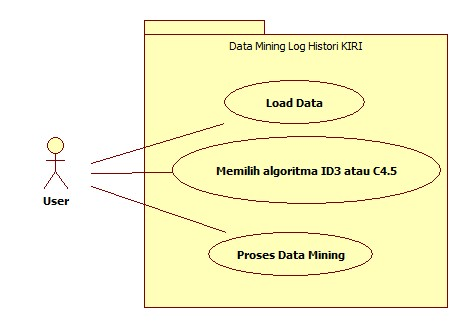
\includegraphics[scale=1]{Gambar/usecase.jpg}
\caption[Diagram \textsl{Use Case} Perangkat Lunak \textsl{Data Mining Log} Histori KIRI]{Diagram \textsl{Use Case} Perangkat Lunak \textsl{Data Mining Log} Histori KIRI} 
\label{fig:diagramUseCase}
\end{figure}

\begin{table}[H]
\caption{Skenario Melakukan \textsl{load} Data}
\begin{tabular}{|l|l|}
\hline
Nama           & Load data                                                       \\ \hline
Aktor          & \textit{User}                                                   \\ \hline
Deskripsi      & Memasukan alamat data yang akan dijadikan sebagai input program \\ \hline
Kondisi awal   & \textsl{Textbox} belum terisi                                   \\ \hline
Kondisi akhir  & \textsl{Textbox} sudah terisi dengan alamat data                \\ \hline
Skenario utama & \textit{User} memasukan alamat data pada textbox                \\ \hline
Eksespi        & Data tidak ditemukan                                            \\ \hline
\end{tabular}
\end{table}

\begin{table}[H]
\caption{Skenario Melakukan \textsl{Data Mining}}
\begin{tabular}{|l|l|}
\hline
Nama           & Proses \textsl{Data Mining }                      								\\ \hline
Aktor          & \textit{User}                                 										\\ \hline
Deskripsi      & Menekan tombol proses pada \textsl{interface}       					    \\ \hline
Kondisi awal   & \textsl{Textbox} belum terisi                          					\\ \hline
Kondisi akhir  & \textsl{Textbox} sudah terisi dengan hasil \textsl{data mining}  \\ \hline
Skenario utama & \textit{User} menekan tombol proses         										  \\ \hline
Eksespi        & Data tidak ditemukan atau data tidak dapat diproses    		  	  \\ \hline
\end{tabular}
\end{table}

\begin{table}[H]
\caption{Skenario Memilih Algoritma yang Akan Digunakan}
\begin{tabular}{|l|l|}
\hline
Nama           & Memilih algoritma ID3 atau C4.5                     \\ \hline
Aktor          & \textit{User}                                       \\ \hline
Deskripsi      & User memilih algoritma yang akan dipakai            \\ \hline
Kondisi awal   & \textsl{Radiobutton} terpilih pada ID3              \\ \hline
Kondisi akhir  & \textsl{Radiobutton} terpilih pada ID3 atau C4.5    \\ \hline
Skenario utama & \textit{User} memilih algoritma yang akan digunakan \\ \hline
Eksespi        & Tidak ada																					 \\ \hline
\end{tabular}
\end{table}


\subsection{Diagram kelas Perangkat Lunak \textsl{Data Mining Log} Histori KIRI}

Pembuatan diagram \textsl{class} untuk memenuhi semua tujuan dari diagram \textsl{use case} dan skenario terdapat pada gambar \ref{fig:classDiagram}.

\begin{figure}[H]
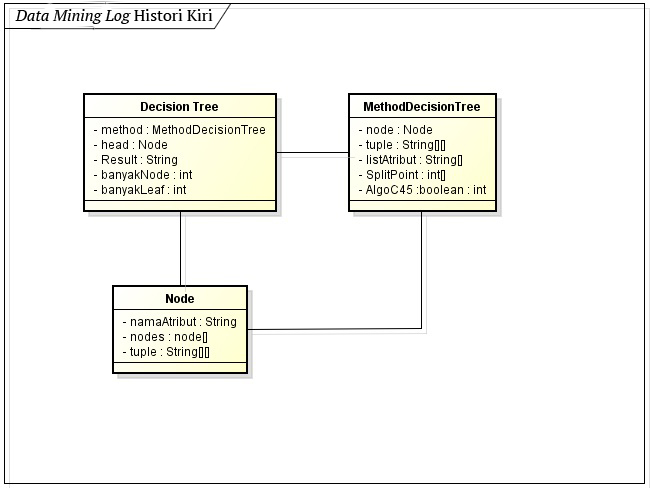
\includegraphics[scale=0.7]{Gambar/classdiagram.jpg}
\caption[Diagram \textsl{Class} Perangkat Lunak \textsl{Data Mining Log} Histori KIRI]{Diagram \textsl{Class} Perangkat Lunak \textsl{Data Mining Log} Histori KIRI} 
\label{fig:classDiagram}
\end{figure}

Berikut deskripsi kelas diagram \textsl{class}:
\begin{itemize}
	\item View, merupakan kelas untuk mengatur desain antar muka.
	\item Controller, merupakan kelas untuk mengatur view dan modul ketika program dijalankan.
	\item CSVReader, merupakan kelas yang memiliki method untuk membaca file dengan format CSV.
	\item ProcessingData, merupakan kelas yang memiliki method untuk melakukan \textsl{preprocessing data}.
	\item DecissionTree, merupakan kelas yang memiliki method untuk membuat \textsl{decision tree} dan menghitung \textsl{confident} dari pohon yang sudah dihasilkan.
	\item DotConverter, merupakan kelas yang memiliki method untuk mengubah \textsl{string} yang merupakan hasil dari kelas DecissionTree (yaitu, \textsl{decision tree} dalam bentuk string) menjadi bahasa dot yang siap dijadikan masukan untuk graphviz.
\end{itemize}
	
















